\documentclass[aspectratio=169]{beamer}
\usepackage[utf8]{inputenc}
\usepackage[T1]{fontenc}
\usepackage{listings}
\usepackage{xcolor}
\usepackage{booktabs}
\usepackage{graphicx}
\usepackage{multirow}
\usepackage{tikz}
\usetikzlibrary{decorations.pathreplacing}
\usepackage{amsmath}
\usepackage{hyperref}

% -- Color Theme (Teal like the app) --
\definecolor{teal}{RGB}{3,107,110}
\definecolor{teallight}{RGB}{3,181,170}
\definecolor{amber}{RGB}{255,183,3}
\definecolor{codebg}{RGB}{245,247,244}
\definecolor{codestring}{RGB}{3,107,110}
\definecolor{codekey}{RGB}{156,39,176}
\definecolor{codecomment}{RGB}{100,100,100}

\usetheme{Madrid}
\usecolortheme[RGB={3,107,110}]{structure}
\setbeamercolor{title}{fg=white}
\setbeamercolor{frametitle}{fg=white,bg=teal}
\setbeamercolor{block title}{bg=teal,fg=white}
\setbeamercolor{block body}{bg=codebg}
\setbeamercolor{alerted text}{fg=amber}
\setbeamerfont{title}{size=\huge}
\setbeamerfont{frametitle}{size=\Large}

% -- Listings Style --
\lstdefinestyle{dartstyle}{
  language={},
  backgroundcolor=\color{codebg},
  basicstyle=\ttfamily\footnotesize,
  keywordstyle=\color{codekey}\bfseries,
  stringstyle=\color{codestring},
  commentstyle=\color{codecomment}\itshape,
  numbers=left,
  numberstyle=\tiny\color{gray},
  breaklines=true,
  frame=single,
  framesep=2mm,
  tabsize=2,
  morekeywords={class,static,final,const,late,required,enum,import,extends,
    implements,abstract,override,Future,Stream,async,await,List,Map,String,
    double,int,bool,void,switch,case,default,for,if,else,return,var,new,as,
    is,show,with,super,this,get,set,factory},
  sensitive=true,
  morestring=[b]',
  morestring=[b]",
}

\lstdefinestyle{pythonstyle}{
  language=Python,
  backgroundcolor=\color{codebg},
  basicstyle=\ttfamily\footnotesize,
  keywordstyle=\color{codekey}\bfseries,
  stringstyle=\color{codestring},
  commentstyle=\color{codecomment}\itshape,
  numbers=left,
  numberstyle=\tiny\color{gray},
  breaklines=true,
  frame=single,
  framesep=2mm,
  tabsize=4,
}

\lstdefinestyle{jsonstyle}{
  language={},
  backgroundcolor=\color{codebg},
  basicstyle=\ttfamily\footnotesize,
  stringstyle=\color{codestring},
  commentstyle=\color{codecomment},
  breaklines=true,
  frame=single,
  framesep=2mm,
  tabsize=2,
}

% -- Title Page --
\title[Environmental IoT Monitoring System]
      {\textbf{Environmental IoT Monitoring System}}
\subtitle{Flutter + MCDM + On-Device ML \\ From Python Notebooks to Cross-Platform App}
\author[Your Name]{Your Name}
\institute[University]{Smart Study Desk Monitor Project}
\date{\today}

\begin{document}

\begin{frame}
  \titlepage
\end{frame}

% -- Outline --
\begin{frame}{Outline}
  \tableofcontents
\end{frame}

% ==========================================================
% PART 0: PROJECT OVERVIEW
% ==========================================================
\section{Project Overview}
\begin{frame}[allowframebreaks]{Project Architecture}
  \begin{columns}
    \column{0.55\textwidth}
    \textbf{Three-Tier Architecture}
    \begin{itemize}
      \item \alert{\textbf{Tier 1: Python}} --- MCDM weight computation \& ML model training
      \item \alert{\textbf{Tier 2: Dart Services}} --- Native MCDM engine, ML inference service
      \item \alert{\textbf{Tier 3: Flutter UI}} --- Cross-platform frontend (Android, iOS, Web, Desktop)
    \end{itemize}

    \vspace{0.3cm}
    \textbf{8 IoT Sensing Domains}
    \begin{columns}
      \column{0.45\textwidth}
      \begin{itemize}
        \item Egg Production
        \item Green Building
        \item Herbal Plant Health
        \item Indoor Air Quality
      \end{itemize}
      \column{0.45\textwidth}
      \begin{itemize}
        \item Smart Library
        \item Building Occupancy
        \item User Behavior (RAED)
        \item IoT Mental Health
      \end{itemize}
    \end{columns}
    \column{0.45\textwidth}
    \begin{block}{Data Flow}
      \centering
      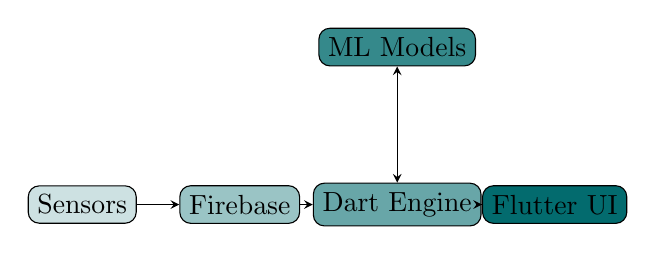
\begin{tikzpicture}[>=stealth, node distance=2cm]
        \node[draw,fill=teal!20,rounded corners] (sensors) {Sensors};
        \node[draw,fill=teal!40,rounded corners,right of=sensors] (fb) {Firebase};
        \node[draw,fill=teal!60,rounded corners,right of=fb] (dart) {Dart Engine};
        \node[draw,fill=teal!80,rounded corners,above of=dart] (ml) {ML Models};
        \node[draw,fill=teal!100,rounded corners,right of=dart] (ui) {Flutter UI};
        \draw[->] (sensors)--(fb);
        \draw[->] (fb)--(dart);
        \draw[<->] (dart)--(ml);
        \draw[->] (dart)--(ui);
      \end{tikzpicture}
    \end{block}
  \end{columns}
\end{frame}

\begin{frame}{What You (The User) Provided}
  \textbf{Your Python work formed the foundation of the entire system:}

  \vspace{0.3cm}
  \begin{block}{8 Jupyter Notebooks}
    Each notebook (\texttt{MCDM\_*.ipynb}) contains:
    \begin{itemize}
      \item Data loading, cleaning, and exploratory analysis
      \item 5 weight method implementations (STD, Entropy, CRITIC, MEREC, Compromise)
      \item 4 scoring formula evaluations (MABAC, MARCOS, SPOTIS, COCOCOMET)
      \item ML model training, hyperparameter tuning, evaluation
      \item Weight tables used as the ``answer key'' for the app
    \end{itemize}
  \end{block}
\end{frame}

\begin{frame}{What You Provided (cont.)}
  \begin{block}{Trained ML Models (\texttt{.pkl} files)}
    \begin{itemize}
      \item \textbf{Egg Production} --- XGBoost ($R^2$=1.00)
      \item \textbf{Green Building} --- Linear Regression ($R^2$=0.003)
      \item \textbf{Herbal Plant Health} --- MLP Classifier (Acc=0.99)
      \item \textbf{IoT Air Quality} --- Linear Regression ($R^2$=0.00)
      \item \textbf{Smart Library} --- MLP Classifier (Acc=0.74)
      \item \textbf{Building Occupancy} --- Random Forest (Acc=0.99)
      \item \textbf{User Behavior RAED} --- Gradient Boosting (Acc=0.86)
      \item \textbf{IoT Mental Health} --- Random Forest ($R^2$=0.52)
    \end{itemize}
  \end{block}
\end{frame}

\begin{frame}{What the Flutter App Adds}
  \textbf{Transformation:} Your Python math is brought to life on users' devices:

  \vspace{0.3cm}
  \begin{columns}
    \column{0.5\textwidth}
    \begin{block}{Offline-First Architecture}
      \begin{itemize}
        \item No server required for MCDM or ML inference
        \item All algorithms rewritten in \alert{native Dart}
        \item Models converted to \alert{pure Dart code} (no TFLite/ONNX)
        \item Real-time predictions on-device in milliseconds
      \end{itemize}
    \end{block}
    \column{0.5\textwidth}
    \begin{block}{Cross-Platform UI}
      \begin{itemize}
        \item Flutter $\rightarrow$ Android, iOS, Web, Windows, macOS, Linux
        \item Config-driven dashboard (JSON defines datasets/sensors)
        \item Per-sensor live/manual toggle, inline editing
        \item Interactive history with \texttt{fl\_chart}
        \item Optional Firebase for data persistence
      \end{itemize}
    \end{block}
  \end{columns}

  \vspace{0.3cm}
  \centering
  \small Your Python $\xrightarrow{\text{m2cgen + custom scripts}}$ Pure Dart $\xrightarrow{\text{Flutter}}$ User's Device
\end{frame}

% ==========================================================
% PART 1: PYTHON - MCDM & ML MODELS
% ==========================================================
\section{Part 1: MCDM \& ML Models in Python}

\begin{frame}[allowframebreaks,fragile]{1.1 MCDM Weight Methods --- Mathematical Foundation}
  \begin{columns}
    \column{0.45\textwidth}
    \small
    \textbf{1. Standard Deviation (STD)}
    \[
    w_j = \frac{\sigma_j}{\sum_{k=1}^n \sigma_k}
    \]
    Higher variance $\Rightarrow$ higher weight

    \vspace{0.2cm}
    \textbf{2. Entropy Method}
    \[
    p_{ij} = \frac{x_{ij}}{\sum_i x_{ij}},\quad
    e_j = -\frac{1}{\ln m}\sum_i p_{ij}\ln p_{ij}
    \]
    \[
    w_j = \frac{1-e_j}{\sum_k (1-e_k)}
    \]
    Lower entropy $\Rightarrow$ lower weight

    \column{0.45\textwidth}
    \small
    \textbf{3. CRITIC Method}
    \[
    C_j = \sigma_j \sum_{k\neq j} (1 - r_{jk})
    \]
    \[
    w_j = \frac{C_j}{\sum_k C_k}
    \]
    High contrast + low correlation $\Rightarrow$ higher weight

    \vspace{0.2cm}
    \textbf{4. MEREC Method}
    Measures impact of removing each criterion on overall performance

    \vspace{0.2cm}
    \textbf{5. Compromise Method}
    \[
    w_j = \frac{\text{STD}_j + \text{Entropy}_j + \text{CRITIC}_j + \text{MEREC}_j}{4}
    \]
  \end{columns}
\end{frame}

\begin{frame}[allowframebreaks,fragile]{1.2 MCDM Scoring Formulas}
  \begin{columns}
    \column{0.5\textwidth}
    \textbf{MABAC}
    \[
    S_i = \sum_{j=1}^n w_j (v_{ij} - \text{BAA}_j)
    \]
    Border Approximation Area comparison

    \vspace{0.3cm}
    \textbf{MARCOS}
    \[
    f(K_i^+, K_i^-) = \frac{K_i^+ + K_i^-}{1 + \frac{1-K_i^+}{K_i^+} + \frac{1-K_i^-}{K_i^-}}
    \]
    Utility degree relative to ideal/anti-ideal

    \column{0.5\textwidth}
    \textbf{SPOTIS}
    \[
    S_i = \sum_{j=1}^n w_j \frac{|x_{ij} - x_j^{\text{ideal}}|}{\text{range}_j}
    \]
    Normalized distance from ideal solution

    \vspace{0.3cm}
    \textbf{COCOCOMET}
    \[
    S_i = \sum_{j=1}^n w_j (1 - |\text{optimal}_j - \text{norm}_{ij}|)
    \]
    Similarity to optimal composite alternative
  \end{columns}
\end{frame}

\begin{frame}[allowframebreaks,fragile]{1.3 Python Training Pipeline --- \texttt{train\_all\_models.py}}
  The Python script that trains all 8 models with a consistent pipeline:

  \begin{lstlisting}[style=pythonstyle]
def normalize_matrix(data, criteria_types):
    normalized_data = data.copy()
    norm_params = {}
    for criterion in data.columns:
        min_val = data[criterion].min()
        max_val = data[criterion].max()
        range_val = max_val - min_val
        norm_params[criterion] = {'min': float(min_val), 'max': float(max_val)}
        if range_val == 0:
            normalized_data[criterion] = 0.5
        else:
            if criteria_types[criterion] == 'cost':
                normalized_data[criterion] = (max_val - data[criterion]) / range_val
            else:
                normalized_data[criterion] = (data[criterion] - min_val) / range_val
    return normalized_data, norm_params
  \end{lstlisting}

  \begin{itemize}
    \item \alert{Cost criteria} (lower is better): temperature, humidity, noise, CO$_2$
    \item \alert{Profit criteria} (higher is better): light, soil moisture, motion
    \item Normalization parameters saved as \texttt{\_norm.pkl} for the app
  \end{itemize}
\end{frame}

\begin{frame}[allowframebreaks,fragile]{1.3 Python Training Pipeline (cont.)}
  \textbf{Eight models, eight training strategies:}

  \vspace{0.2cm}
  \begin{lstlisting}[style=pythonstyle]
# Egg Production: XGBoost Regressor
model = XGBRegressor(n_estimators=100, random_state=42)
model.fit(X_normalized, y)
print(f"$R^2$ = {model.score(X_normalized, y):.4f}")  # 1.0000

# Green Building: Linear Regression
model = LinearRegression()
model.fit(X_normalized, y)
print(f"$R^2$ = {model.score(X_normalized, y):.4f}")  # 0.0028

# Herbal Plant Health: MLP Classifier (64,32)
model = MLPClassifier(hidden_layer_sizes=(64, 32), max_iter=500)
model.fit(X_normalized, y)
print(f"Accuracy = {model.score(X_normalized, y):.4f}")  # 0.9900
  \end{lstlisting}

  \begin{itemize}
    \item Each model saved as \texttt{.pkl} + \texttt{\_norm.pkl} (normalization params) + optional \texttt{\_classes.pkl}
    \item Classification models store class label mappings (e.g., \texttt{Healthy}/\texttt{Unhealthy})
  \end{itemize}
\end{frame}

\begin{frame}[allowframebreaks,fragile]{1.4 Compact Models --- Strategic Retraining}
  \textbf{Problem:} m2cgen doesn't support GradientBoostingClassifier.
  \textbf{Solution:} Retrain RAED with RandomForest.

  \vspace{0.2cm}
  \begin{lstlisting}[style=pythonstyle]
# train_compact_models.py
# Retrain with reduced tree count for manageable Dart file sizes

# Building Occupancy: 100 -> 20 trees, depth 8
model = RandomForestClassifier(
    n_estimators=20, max_depth=8, random_state=42, n_jobs=-1
)
Accuracy unchanged ~ 0.99

# User Behavior RAED: GB -> RF, 10 trees, depth 8
model = RandomForestClassifier(
    n_estimators=10, max_depth=8, random_state=42, n_jobs=-1
)
Accuracy 0.8577

# IoT Mental Health: 100 -> 20 trees, depth 10
model = RandomForestRegressor(
    n_estimators=20, max_depth=10, random_state=42, n_jobs=-1
)
$R^2$ unchanged ~ 0.52
  \end{lstlisting}
\end{frame}

\begin{frame}[allowframebreaks,fragile]{1.5 Weight Extraction --- From Notebooks to Config}
  \textbf{Every notebook computes 5 weight vectors $\times$ 8 datasets = 40 weight entries.}
  These were extracted and embedded into the Flutter config:

  \vspace{0.2cm}
  \begin{lstlisting}[style=jsonstyle]
{
  "id": "egg_production",
  "weights": {
    "std":       [0.1072, 0.1266, 0.1379, ...],
    "entropy":   [0.0981, 0.1154, 0.1482, ...],
    "critic":    [0.1123, 0.1301, 0.1425, ...],
    "merec":     [0.0924, 0.1108, 0.1337, ...],
    "compromise":[0.1025, 0.1207, 0.1406, ...]
  }
}
  \end{lstlisting}

  \begin{itemize}
    \item Each dataset has a \texttt{modelConfig} sub-object (type, target, class labels)
    \item Each sensor has a \texttt{modelFeature} mapping linking sensor $\rightarrow$ ML feature name
    \item Weights verified 100\% matching notebook output during development
  \end{itemize}
\end{frame}

% ==========================================================
% PART 2: MCDM in DART
% ==========================================================
\section{Part 2: MCDM Implementation in Dart}

\begin{frame}[allowframebreaks,fragile]{2.1 Python $\rightarrow$ Dart Translation Strategy}
  \textbf{The core challenge:} Rewrite all MCDM math from Python (NumPy/pandas) into pure Dart.

  \vspace{0.3cm}
  \begin{columns}
    \column{0.45\textwidth}
    \textbf{Python (numpy)}
    \begin{lstlisting}[style=pythonstyle]
import numpy as np
stds = np.std(matrix, axis=0)
weights = stds / stds.sum()
    \end{lstlisting}

    \column{0.45\textwidth}
    \textbf{Dart (pure)}
    \begin{lstlisting}[style=dartstyle]
List<double> stds = List.filled(n, 0.0);
for (int j = 0; j < n; j++) {
  double mean = 0;
  for (int i = 0; i < m; i++) mean += matrix[i][j];
  mean /= m;
  double var = 0;
  for (int i = 0; i < m; i++) var += pow(matrix[i][j] - mean, 2);
  var /= m;
  stds[j] = sqrt(var);
}
double sum = stds.reduce((a, b) => a + b);
return stds.map((s) => s / sum).toList();
    \end{lstlisting}
  \end{columns}

  \vspace{0.3cm}
  \centering
  \alert{Result:} Mathematically identical, runs natively on device (no server needed!)
\end{frame}

\begin{frame}[allowframebreaks,fragile]{2.2 The MCDM Engine --- \texttt{mcdm\_calculator.dart}}
  \textbf{Core service:} 5 weight methods + 4 scoring formulas + normalization.

  \vspace{0.1cm}
  \begin{lstlisting}[style=dartstyle,basicstyle=\ttfamily\footnotesize]
enum WeightMethod { std, entropy, critic, merec, compromise }
enum ScoringMethod { mabac, marcos, spotis, cococomet }

class MCDMCalculator {
  static List<List<double>> normalizeSensorMatrix(...) { ... }
  static List<double> computeStdWeights(...)      { ... }
  static List<double> computeEntropyWeights(...)  { ... }
  static List<double> computeCriticWeights(...)   { ... }
  static List<double> computeMerecWeights(...)    { ... }
  static List<double> computeCompromiseWeights(...) { ... }
  static List<double> computeMabacScore(...)      { ... }
  static List<double> computeMarcosScore(...)     { ... }
  static List<double> computeSpotisScore(...)     { ... }
  static List<double> computeCocometScore(...)    { ... }
}
  \end{lstlisting}
\end{frame}

\begin{frame}[allowframebreaks]{2.2 MCDM Architecture --- 3 Calculator Layers}
  \begin{itemize}
    \item \texttt{\textbf{MCDMCalculator}} --- batch matrix analysis on historical data rows
    \item \texttt{\textbf{PreCalculatedMCDMCalculator}} --- single-reading analysis using notebook-embedded weights
    \item \texttt{\textbf{FlexibleMCDMCalculator}} --- dynamic weight computation for any number of sensors
  \end{itemize}

  \vspace{0.4cm}
  \begin{block}{Key Design Decision}
    \alert{Single reading $\ne$ variance.} Dynamic weights from one reading are meaningless.
    Pre-calculated weights from notebooks guarantee mathematically correct results.
  \end{block}
\end{frame}

\begin{frame}[allowframebreaks,fragile]{2.3 Weight Methods --- Entropy in Dart}
  \begin{lstlisting}[style=dartstyle,basicstyle=\ttfamily\footnotesize]
static List<double> computeEntropyWeights(
    List<List<double>> matrix) {
  int n = matrix[0].length;
  List<double> entropies = List.filled(n, 0.0);
  for (int j = 0; j < n; j++) {
    double sum = 0;
    for (int i = 0; i < matrix.length; i++)
      sum += matrix[i][j];
    double entropy = 0;
    for (int i = 0; i < matrix.length; i++) {
      double p = matrix[i][j] / sum;
      if (p > 0) entropy += p * log(p);
    }
    entropy = -entropy / log(matrix.length);
    entropies[j] = entropy;
  }
  double total = entropies
      .map((e) => 1 - e).reduce((a, b) => a + b);
  return entropies
      .map((e) => (1 - e) / total).toList();
}
  \end{lstlisting}
\end{frame}

\begin{frame}[allowframebreaks,fragile]{2.3 Weight Methods --- CRITIC in Dart}
  \begin{lstlisting}[style=dartstyle,basicstyle=\ttfamily\footnotesize]
static List<double> computeCriticWeights(
    List<List<double>> matrix) {
  // Normalize -> compute stds ->
  // correlation matrix -> contrast
  List<double> contrast =
      List.filled(critCount, 0.0);
  for (int j = 0; j < critCount; j++) {
    double sumCorr = 0;
    for (int k = 0; k < critCount; k++)
      if (j != k)
        sumCorr += 1 - pearsonCorrelation(
            normalized, j, k);
    contrast[j] = stds[j] * sumCorr;
  }
  double total = contrast
      .reduce((a, b) => a + b);
  return contrast
      .map((c) => c / total).toList();
}
  \end{lstlisting}
\end{frame}

\begin{frame}[allowframebreaks,fragile]{2.4 Pre-Calculated Weights Approach}
  \textbf{For real-time single-readings, we use pre-computed weights from the notebooks:}

  \vspace{0.2cm}
  \texttt{PreCalculatedMCDMCalculator} loads weights from \texttt{mcdm\_flutter\_config.json}:

  \vspace{0.2cm}
  \begin{lstlisting}[style=dartstyle]
static double calculateScore({
  required List<LiveMetricValue> sensorValues,
  required LiveMetricDataset dataset,
  required String weightMethod,
  String scoringMethod = 'MABAC',
}) {
  final weights = dataset.getWeights(weightMethod);
  // Normalize values, apply weights, compute score
  ...
  switch (scoringMethod) {
    case 'MABAC':    return _scoreMABAC(vals, wts);
    case 'MARCOS':   return _scoreMARCOS(vals, wts);
    case 'SPOTIS':   return _scoreSPOTIS(vals, wts);
    case 'COCOCOMET': return _scoreCOCOCOMET(vals, wts);
  }
}
  \end{lstlisting}

  \textbf{Why?} Dynamically computing weights from a single reading is meaningless
  (need variance across alternatives). Pre-calculated weights = notebook-verified accuracy.
\end{frame}

\begin{frame}[allowframebreaks,fragile]{2.5 Scoring Formulas --- Adapted for Per-Row [0,1]}
  The Flutter scoring uses \alert{adapted per-row versions} (not batch ranking from notebooks):

  \begin{columns}
    \column{0.5\textwidth}
    \textbf{MABAC (Quadratic)}
    \begin{lstlisting}[style=dartstyle]
static double _scoreMABAC(
    List<double> vals, List<double> wts) {
  double sumW = 0, sumV2 = 0;
  for (int i = 0; i < vals.length; i++) {
    sumW += wts[i];
    sumV2 += wts[i] * vals[i] * vals[i];
  }
  return (sumW > 0 ? sumV2 / sumW : 0.5)
      .clamp(0.0, 1.0);
}
    \end{lstlisting}

    \column{0.5\textwidth}
    \textbf{MARCOS (Linear)}
    \begin{lstlisting}[style=dartstyle]
static double _scoreMARCOS(
    List<double> vals, List<double> wts) {
  double sumW = 0, sumV = 0;
  for (int i = 0; i < vals.length; i++) {
    sumW += wts[i];
    sumV += wts[i] * vals[i];
  }
  return (sumW > 0 ? sumV / sumW : 0.5)
      .clamp(0.0, 1.0);
}
    \end{lstlisting}
  \end{columns}

  \vspace{0.2cm}
  \centering
  \alert{All 4 produce mathematically distinct scores (verified: changing method changes result)}
\end{frame}

\begin{frame}[allowframebreaks,fragile]{2.5 Scoring Formulas (cont.)}
  \begin{columns}
    \column{0.5\textwidth}
    \textbf{SPOTIS (Exponential Decay)}
    \begin{lstlisting}[style=dartstyle]
static double _scoreSPOTIS(
    List<double> vals, List<double> wts) {
  double sumW = 0, distSq = 0;
  for (int i = 0; i < vals.length; i++) {
    sumW += wts[i];
    distSq += wts[i] * vals[i] * vals[i];
  }
  final dist = sqrt(
      sumW > 0 ? distSq / sumW : 0);
  return exp(-dist).clamp(0.0, 1.0);
  // Minimum ~ exp(-1) = 0.368
}
    \end{lstlisting}

    \column{0.5\textwidth}
    \textbf{COCOCOMET (Geometric $\times$ Arithmetic)}
    \begin{lstlisting}[style=dartstyle]
static double _scoreCOCOCOMET(
    List<double> vals, List<double> wts) {
  double sumW = 0, sumV = 0;
  double product = 1.0;
  for (int i = 0; i < vals.length; i++) {
    sumW += wts[i];
    sumV += wts[i] * vals[i];
    product *= pow(max(vals[i], 1e-10), wts[i]);
  }
  final weightedAvg = sumV / sumW;
  return (product * (1.0 + weightedAvg) / 2.0)
      .clamp(0.0, 1.0);
}
    \end{lstlisting}
  \end{columns}
\end{frame}

\begin{frame}[allowframebreaks]{2.6 Service Architecture --- Complete Picture}
  \centering
  \textbf{Three MCDM Calculators, One Goal}

  \vspace{0.3cm}
  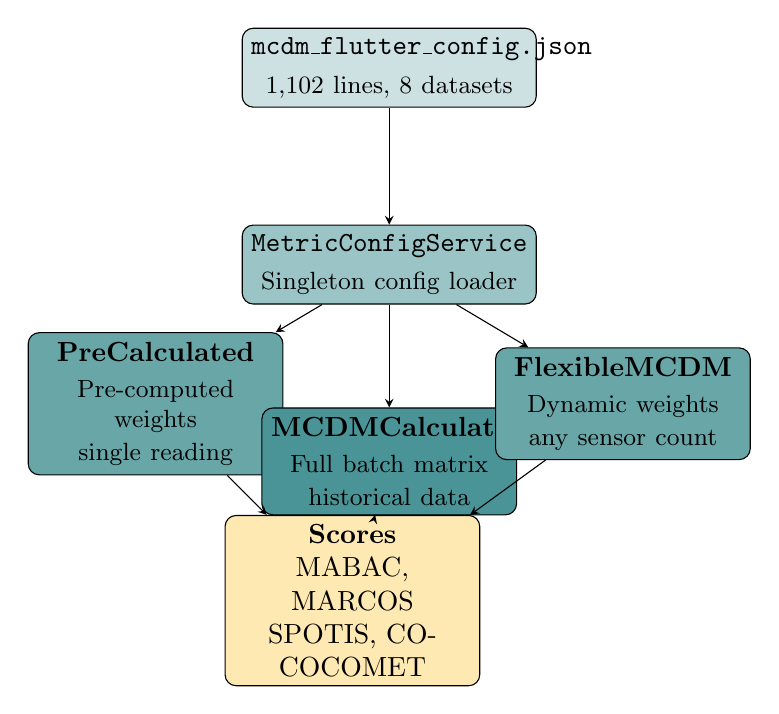
\begin{tikzpicture}[>=stealth, node distance=2.5cm]
    \node[draw,fill=teal!20,rounded corners,text width=3.5cm,align=center] (config)
      {\texttt{mcdm\_flutter\_config.json}\\[2pt]\small 1,102 lines, 8 datasets};
    \node[draw,fill=teal!40,rounded corners,below of=config,text width=3.5cm,align=center] (metriccfg)
      {\texttt{MetricConfigService}\\[2pt]\small Singleton config loader};
    \node[draw,fill=teal!60,rounded corners,below left of=metriccfg,xshift=-1.2cm,text width=3cm,align=center] (precalc)
      {\textbf{PreCalculated}\\[2pt]\small Pre-computed weights\\single reading};
    \node[draw,fill=teal!72,rounded corners,below of=metriccfg,text width=3cm,align=center] (full)
      {\textbf{MCDMCalculator}\\[2pt]\small Full batch matrix\\historical data};
    \node[draw,fill=teal!60,rounded corners,below right of=metriccfg,xshift=1.2cm,text width=3cm,align=center] (flex)
      {\textbf{FlexibleMCDM}\\[2pt]\small Dynamic weights\\any sensor count};
    \node[draw,fill=amber!30,rounded corners,below of=precalc,xshift=2.5cm,text width=3cm,align=center] (score)
      {\textbf{Scores}\\MABAC, MARCOS\\SPOTIS, COCOCOMET};

    \draw[->] (config) -- (metriccfg);
    \draw[->] (metriccfg) -- (precalc);
    \draw[->] (metriccfg) -- (full);
    \draw[->] (metriccfg) -- (flex);
    \draw[->] (precalc) -- (score);
    \draw[->] (full) -- (score);
    \draw[->] (flex) -- (score);
  \end{tikzpicture}
\end{frame}

% ==========================================================
% PART 3: ML MODELS RUNNING LOCALLY IN DART
% ==========================================================
\section{Part 3: On-Device ML Inference in Dart}

\begin{frame}[allowframebreaks,fragile]{3.1 The Model Conversion Pipeline}
  \textbf{How Python $\rightarrow$ Dart?} Two strategies depending on model type:

  \vspace{0.3cm}
  \begin{columns}
    \column{0.55\textwidth}
    \textbf{Strategy A: m2cgen (6 models)}
    \begin{lstlisting}[style=pythonstyle]
import m2cgen as m2c

model = joblib.load('models/egg_production.pkl')
code = m2c.export_to_dart(
    model,
    function_name='predictEggproduction'
)
with open('egg_production.dart', 'w') as f:
    f.write(code)
    \end{lstlisting}
    Supports: XGBoost, RandomForest, LinearRegression

    \column{0.45\textwidth}
    \textbf{Strategy B: Custom exporter (2 MLPs)}
    \begin{lstlisting}[style=pythonstyle]
def export_mlp_to_dart(model, input_names,
                       class_names, function_name):
    # Extract weights/biases
    weights = model.coefs_
    biases = model.intercepts_
    # Generate: ReLU forward pass
    # + softmax (multi-class)
    # + sigmoid (binary)
    # + score (regression)
    \end{lstlisting}
    Supports: MLPClassifier, MLPRegressor
  \end{columns}

  \vspace{0.3cm}
  \textbf{Output:} 8 Dart files in \texttt{lib/generated\_models/*.dart}
\end{frame}

\begin{frame}[allowframebreaks,fragile]{3.2 Example: XGBoost $\rightarrow$ Dart (Egg Production)}
  \texttt{m2cgen} converts XGBoost decision trees into nested if-else chains:

  \begin{lstlisting}[style=dartstyle]
double predictEggproduction(List<double> input) {
  double var;
  if (input[5] <= 0.49027279019355774) {
    if (input[2] <= 0.28947368264198303) {
      ...
    }
  } else {
    if (input[0] <= 0.17105263471603394) {
      ...
    }
  }
  return var;  // Predicted egg count
}
  \end{lstlisting}

  \vspace{0.2cm}
  \begin{itemize}
    \item Trees are flattened into sequential if-else (interpreted as decision paths)
    \item ~58,000 characters for Egg Production XGBoost
    \item RF models: ~55,000 chars each (20 trees $\times$ depth 8)
    \item Linear regression: just 3 lines ($y = \beta_0 + \sum \beta_i x_i$)
  \end{itemize}
\end{frame}

\begin{frame}[allowframebreaks,fragile]{3.3 Example: MLP $\rightarrow$ Dart (Herbal Plant Health)}
  \texttt{export\_mlp\_to\_dart.py} generates ReLU + softmax forward pass:

  \begin{lstlisting}[style=dartstyle,basicstyle=\ttfamily\footnotesize]
double predictHerbalPlantHealth(List<double> input) {
  final weights0 = <List<double>>[ ... ]; // 4x60 matrix
  final biases0 = <double>[0.0, 0.0, ...]; // 60 biases

  // Hidden layer: 4 -> 60 with ReLU
  List<double> h1 = List.filled(60, 0.0);
  for (int j = 0; j < 60; j++) {
    double s = biases0[j];
    for (int k = 0; k < input.length; k++)
      s += input[k] * weights0[k][j];
    h1[j] = s > 0 ? s : 0.0;  // ReLU
  }

  // Output layer: 60 -> 2 with softmax
  List<double> output = List.filled(2, 0.0);
  // ... weighted sum ...
  // softmax: return class index 0 (Healthy) or 1 (Unhealthy)
}
  \end{lstlisting}

  \vspace{0.1cm}
  \small MLP architecture: 4 inputs $\rightarrow$ 60 hidden (ReLU) $\rightarrow$ 2 output (softmax)
\end{frame}

\begin{frame}[allowframebreaks,fragile]{3.4 Model Predictor --- The Central Router}
  \texttt{model\_predictor.dart} routes all 8 dataset predictions:

  \vspace{0.1cm}
  \begin{lstlisting}[style=dartstyle,basicstyle=\ttfamily\footnotesize]
class ModelPredictor {
  static Future<void> loadNormalization() async { ... }

  static double predict(String datasetId,
      Map<String, double> sensorValues) {
    final features = getModelFeatures(datasetId);
    final input = <double>[];
    for (final feature in features) {
      final normVal = _normalize(datasetId, feature,
          sensorValues[feature] ?? 0.5);
      input.add(normVal.clamp(0.0, 1.0));
    }
    switch (datasetId) {
      case 'egg_production':   return predictEggproduction(input);
      case 'green_building':   return predictGreenbuilding(input);
      case 'building_occupancy': return _argmax(predictBuildingoccupancy(input));
      case 'user_behavior_raed': return _argmax(predictUserBehaviorRaed(input));
      default: return 0;
    }
  }
}
  \end{lstlisting}
\end{frame}

\begin{frame}[allowframebreaks,fragile]{3.4 Model Predictor --- Normalization \& Dispatch}
  \textbf{Normalization:} Same cost/profit logic as Python training.

  \vspace{0.1cm}
  \begin{lstlisting}[style=dartstyle,basicstyle=\ttfamily\footnotesize]
static double _normalize(String datasetId,
    String featureName, double rawValue) {
  // Load min/max from model_normalization.json
  final range = maxVal - minVal;
  final isCost = featureName.toLowerCase()
      .contains('temperature') || ...
  if (isCost)
    return (maxVal - rawValue) / range;  // lower is better
  else
    return (rawValue - minVal) / range;  // higher is better
}
  \end{lstlisting}

  \vspace{0.1cm}
  \begin{itemize}
    \item Classification models: \texttt{\_argmax()} returns class index
    \item \texttt{predictLabel()} maps index to class name via \texttt{model\_normalization.json}
    \item All 8 generated models imported, dispatched via \texttt{switch}
  \end{itemize}
\end{frame}

\begin{frame}[allowframebreaks,fragile]{3.5 Normalization: The Critical Bridge}
  \textbf{Models were trained on normalized data $\Rightarrow$ predictions need normalized inputs}
  \texttt{assets/model\_normalization.json} stores per-dataset, per-feature min/max:

  \vspace{0.1cm}
  \begin{lstlisting}[style=jsonstyle,basicstyle=\ttfamily\footnotesize]
{
  "normalization": {
    "egg_production": {
      "Temperature": {"min": 10.0, "max": 35.0},
      "Humidity": {"min": 20.0, "max": 80.0},
      "Light_Intensity": {"min": 0.0, "max": 500.0}
    },
    ...
  },
  "classes": {
    "herbal_plant_health": ["Healthy", "Unhealthy"],
    "smart_library": ["Critical", "Optimal", "Sub Optimal"],
    "building_occupancy": ["Absent", "Present"],
    "user_behavior_raed": ["eating","sleeping","stressed","studying","walking"]
  }
}
  \end{lstlisting}
\end{frame}

\begin{frame}[allowframebreaks,fragile]{3.5 Normalization Logic \& Export Pipeline}

  \textbf{Normalization logic:}
  \begin{itemize}
    \item \alert{Cost} (lower better): $\frac{max - raw}{max - min}$
    \item \alert{Profit} (higher better): $\frac{raw - min}{max - min}$
    \item Clamped to [0.0, 1.0], same exact parameters as Python training
  \end{itemize}

  \vspace{0.2cm}
  \textbf{Export pipeline (Python $\rightarrow$ JavaScript):}
  \begin{lstlisting}[style=pythonstyle,basicstyle=\ttfamily\footnotesize]
# export_norm_params.py
for name in datasets:
    norm_params = joblib.load(f'trained_models/{name}_norm.pkl')
    # Convert numpy -> native Python types
    # Write to model_normalization.json
    \end{lstlisting}
\end{frame}

\begin{frame}[allowframebreaks,fragile]{3.6 Complete ML Data Flow}
  \centering
  \large \textbf{From sensor to prediction in under 50ms (on-device)}

  \vspace{0.3cm}
  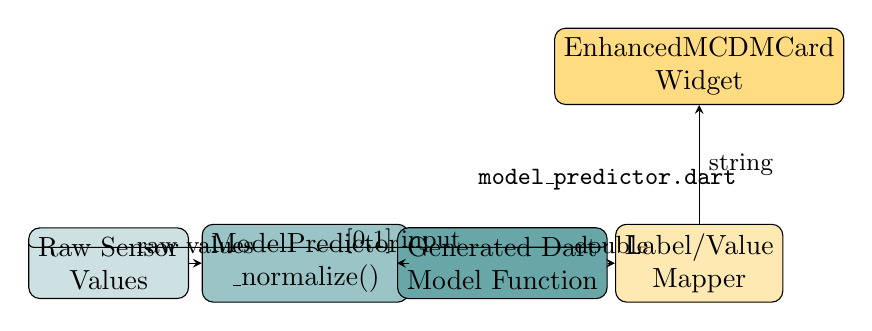
\begin{tikzpicture}[>=stealth, node distance=2.5cm]
    \node[draw,fill=teal!20,rounded corners,align=center] (raw)
      {Raw Sensor\\Values};
    \node[draw,fill=teal!40,rounded corners,right of=raw,align=center] (norm)
      {ModelPredictor\\\_normalize()};
    \node[draw,fill=teal!60,rounded corners,right of=norm,align=center] (model)
      {Generated Dart\\Model Function};
    \node[draw,fill=amber!30,rounded corners,right of=model,align=center] (label)
      {Label/Value\\Mapper};
    \node[draw,fill=amber!50,rounded corners,above of=label,align=center] (ui)
      {EnhancedMCDMCard\\Widget};

    \draw[->] (raw) -- node[above]{\small raw values} (norm);
    \draw[->] (norm) -- node[above]{\small [0,1] input} (model);
    \draw[->] (model) -- node[above]{\small double} (label);
    \draw[->] (label) -- node[right]{\small string} (ui);

    \draw[decorate,decoration={brace,mirror,raise=6pt}]
      (raw.north west) -- (model.north east)
      node[above,yshift=10pt]{\small \texttt{model\_predictor.dart}};
  \end{tikzpicture}

  \vspace{0.3cm}
  \begin{block}{Key Principle}
    MCDM weights and ML predictions are \alert{completely independent} calculations.
    Changing weight/scoring method does NOT change model predictions
    (internally fixed to Compromise weights + MARCOS scoring).
  \end{block}
\end{frame}

% ==========================================================
% PART 4: FRONTEND
% ==========================================================
\section{Part 4: Frontend --- Flutter UI \& Firebase}

\begin{frame}[allowframebreaks,fragile]{4.1 main.dart --- Bootstrap}
  \begin{lstlisting}[style=dartstyle,basicstyle=\ttfamily\footnotesize]
Future<void> main() async {
  WidgetsFlutterBinding.ensureInitialized();
  // 1. Load MCDM config JSON
  final configJson = await rootBundle
      .loadString('mcdm_flutter_config.json');
  MetricConfigService().loadFromJson(configJson);
  // 2. Initialize Firebase
  await Firebase.initializeApp(
    options: DefaultFirebaseOptions.currentPlatform,
  );
  // 3. Launch app with Firebase repo
  runApp(App(
    repository: FirebaseDataRepository(),
    firebaseReady: true,
  ));
}
  \end{lstlisting}
\end{frame}

\begin{frame}[allowframebreaks,fragile]{4.1 app.dart --- MaterialApp Theme}
  \begin{lstlisting}[style=dartstyle,basicstyle=\ttfamily\footnotesize]
class _AppState extends State<App> {
  @override
  Widget build(BuildContext context) {
    final colorScheme = ColorScheme.fromSeed(
      seedColor: const Color(0xFF036B6E),
    );
    return MaterialApp(
      title: 'Smart Study Desk Monitor',
      theme: ThemeData(
        colorScheme: colorScheme,
        useMaterial3: true,
        textTheme: GoogleFonts.spaceGroteskTextTheme(),
      ),
      home: DashboardScreen(
        repository: widget.repository,
        firebaseReady: widget.firebaseReady,
      ),
    );
  }
}
  \end{lstlisting}
  \vspace{0.1cm}
  \small Teal scheme (\#036B6E), SpaceGrotesk font, Material3
\end{frame}

\begin{frame}[allowframebreaks,fragile]{4.2 Firebase Configuration}
  \texttt{firebase\_options.dart} --- Per-platform Firebase initialization:

  \vspace{0.1cm}
  \begin{lstlisting}[style=dartstyle,basicstyle=\ttfamily\footnotesize]
class DefaultFirebaseOptions {
  static FirebaseOptions get currentPlatform { ... }

  static FirebaseOptions get android => FirebaseOptions(
    apiKey: 'AIzaSy...',
    appId: '1:...:android:...',
    projectId: 'smart-study-desk-monitor',
    databaseURL: 'https://...europe-west1.firebasedatabase.app',
  );
  // iOS, Web, Windows, macOS, Linux -- each with platform-specific keys
}
  \end{lstlisting}
\end{frame}

\begin{frame}[allowframebreaks]{4.2 Firebase Data Repository}
  \textbf{Streams from Firebase Realtime Database:}
  \begin{itemize}
    \item \texttt{study\_desk\_monitor/\textbf{readings}} --- Real-time sensor data (temp, humidity, noise, light)
    \item \texttt{study\_desk\_monitor/\textbf{alerts}} --- System alerts
    \item \texttt{study\_desk\_monitor/settings/\textbf{thresholds}} --- Configurable limits
    \item \texttt{study\_desk\_monitor/\textbf{mcdm\_analysis}} --- Stored MCDM results
  \end{itemize}

  \vspace{0.3cm}
  \begin{block}{Graceful Degradation}
    If Firebase fails to initialize, the app continues without it.
    Mock data repository provides test data for development.
  \end{block}
\end{frame}

\begin{frame}[allowframebreaks,fragile]{4.3 Data Models --- lib/models/}
  8 model files, each mapping 1:1 to the CSV datasets:

  \vspace{0.2cm}
  \begin{lstlisting}[style=dartstyle]
class SensorReadings {
  Map<String, double?> values;  // sensorId -> value
  InputMode mode;               // firebase | manual

  bool hasAllRequiredSensors(List<String> required);
  List<double> toList();  // ordered values for MCDM
}

class DatasetConfig {
  String id, name, description;
  Map<String, SensorConfig> sensors;  // sensorId -> config
  List<String> requiredSensorIds;
}

class SensorConfig {
  String id, displayName, unit;
  double minValue, maxValue, meanValue;
  CriteriaType criteriaType;  // cost | profit
  String? modelFeature;       // ML feature name mapping
}
  \end{lstlisting}

  \textbf{Consistent pattern:} \texttt{fromJson()}, \texttt{toJson()}, \texttt{toList()} on every model.
\end{frame}

\begin{frame}[allowframebreaks,fragile]{4.4 Screens Overview}
  4 screens, each with a clear responsibility:

  \vspace{0.3cm}
  \begin{columns}
    \column{0.5\textwidth}
    \textbf{\texttt{dashboard\_screen.dart}} (main)
    \begin{itemize}
      \item Dataset selector (8 choices)
      \item Connection status indicator
      \item Stat cards (temperature, humidity, noise, light)
      \item \alert{EnhancedMCDMCard}: weight/scoring selectors, ML prediction
      \item Navigate to History
    \end{itemize}

    \column{0.5\textwidth}
    \textbf{\texttt{history\_screen.dart}}
    \begin{itemize}
      \item \texttt{fl\_chart} line charts (4 sensors)
      \item 200 historical readings
      \item Y-axis labels + HH:mm X-axis time labels
      \item Touch tooltips
      \item Scrollable past readings
    \end{itemize}
  \end{columns}

  \vspace{0.3cm}
  \begin{columns}
    \column{0.5\textwidth}
    \textbf{\texttt{live\_metrics\_dashboard\_screen.dart}}
    \begin{itemize}
      \item Config-driven metric editor
      \item Per-sensor live/manual toggle
      \item MCDM score display (all 4 methods)
      \item Stress prediction (V2 model)
    \end{itemize}

    \column{0.5\textwidth}
    \textbf{\texttt{mcdm\_analysis\_screen.dart}}
    \begin{itemize}
      \item Dedicated MCDM analysis
      \item Full weight/scoring method selection
      \item Firebase persistence of results
      \item Stress prediction card
    \end{itemize}
  \end{columns}
\end{frame}

\begin{frame}[allowframebreaks,fragile]{4.5 Widgets --- Reusable UI Components}
  15 widgets in \texttt{lib/widgets/}:

  \vspace{0.3cm}
  \begin{columns}
    \column{0.33\textwidth}
    \textbf{Data Display}
    \begin{itemize}
      \item \texttt{StatCard}
      \item \texttt{ConnectionPill}
      \item \texttt{ComfortGauge}
      \item \texttt{LineChartCard}
      \item \texttt{SectionHeader}
    \end{itemize}

    \column{0.33\textwidth}
    \textbf{MCDM Related}
    \begin{itemize}
      \item \texttt{EnhancedMCDMCard} (608 lines)
      \item \texttt{MCDMScoreCard}
      \item \texttt{MCDMDashboardCard}
      \item \texttt{LastMetricWidget}
      \item \texttt{DatasetSelector}
    \end{itemize}

    \column{0.33\textwidth}
    \textbf{Interaction \& Alerts}
    \begin{itemize}
      \item \texttt{MetricEditorWidget}
      \item \texttt{MultiSensorInputWidget}
      \item \texttt{StressPredictionCard}
      \item \texttt{AlertPanel}
      \item \texttt{ThresholdsCard}
    \end{itemize}
  \end{columns}

  \vspace{0.2cm}
  All consume sensor data from \texttt{Reading} or \texttt{SensorReadings} models
  and delegate computation to the service layer.
\end{frame}

\begin{frame}[allowframebreaks]{4.6 The EnhancedMCDMCard --- Integration Hub}
  \textbf{The 608-line widget connecting user interaction $\rightarrow$ MCDM $\rightarrow$ ML:}

  \vspace{0.2cm}
  \begin{block}{Build Flow}
    \begin{enumerate}
      \item \textbf{DatasetSelector} --- Pick one of 8 datasets
      \item \textbf{Weight/Scoring chips} --- Choose from 5 weight + 4 scoring methods
      \item \textbf{Sensor editor} --- Per-sensor: use live Firebase value \textit{or} manual override
      \item \textbf{MCDM score} --- \texttt{PreCalculatedMCDMCalculator.calculateScore()} with progress bar
      \item \textbf{ML prediction} --- \texttt{ModelPredictor.predict()} + class label
      \item \textbf{Description/Range} --- \texttt{getPredictionDescription()} explains what the value means
    \end{enumerate}
  \end{block}
\end{frame}

\begin{frame}[allowframebreaks,fragile]{4.7 Config-Driven Architecture}
  \textbf{Entire app driven by \texttt{mcdm\_flutter\_config.json} (1102 lines).}

  \vspace{0.1cm}
  \begin{lstlisting}[style=jsonstyle,basicstyle=\ttfamily\footnotesize]
{
  "version": "2.0",
  "datasets": [
    {
      "id": "egg_production",
      "name": "Egg Production Analysis",
      "predictionType": "REGRESSION",
      "sensors": [
        {
          "id": "temp", "name": "temperature",
          "displayName": "Temperature (C)", "type": "COST",
          "range": {"min": 10.0, "max": 35.0},
          "weight": 0.1072, "modelFeature": "Temperature"
        }, ...
      ],
      "weights": {
        "std": [0.1072, 0.1266, ...],
        "entropy": [0.0981, 0.1154, ...],
        "compromise": [0.1025, 0.1207, ...]
      },
      "modelConfig": {
        "type": "model",
        "target": "Total_egg_production",
        "modelFeatures": ["Temperature", "Humidity", ...]
      }
    }  // + 7 more datasets
  ]
}
  \end{lstlisting}
\end{frame}

\begin{frame}[allowframebreaks]{4.8 Services Layer (lib/services/) --- Data \& Config}
  \small
  \textbf{Data Access:}
  \texttt{data\_repository.dart} (interface) | \texttt{firebase\_data\_repository.dart} (RTDB) | \texttt{mock\_data\_repository.dart} (test)

  \vspace{0.1cm}
  \textbf{Configuration:}
  \texttt{metric\_config\_service.dart} (JSON loader) | \texttt{config\_service.dart} (typed access)

  \vspace{0.1cm}
  \textbf{MCDM (5 files):}
  \texttt{mcdm\_calculator.dart} (batch, 600 lines) | \texttt{mcdm\_calculator\_simple.dart} (pre-calc) | \texttt{precalculated\_mcdm\_calculator.dart} (live) | \texttt{flexible\_mcdm\_calculator.dart} (dynamic) | \texttt{mcdm\_service.dart} (Firebase persist)

  \vspace{0.1cm}
  \textbf{ML:}
  \texttt{model\_predictor.dart} (router) | \texttt{model\_inference\_service.dart} (legacy)

  \vspace{0.1cm}
  \textbf{Derived Metrics (8 files):}
  \texttt{normalization\_service.dart} | \texttt{comfort\_score\_service.dart} (ASHRAE) | \texttt{stress\_prediction\_model.dart} (V1) + \texttt{\_v2.dart} | \texttt{alert\_service.dart} | \texttt{data\_aggregation\_service.dart} | \texttt{sensor\_simulation\_service.dart} | \texttt{visualization\_service.dart}
\end{frame}

\begin{frame}[allowframebreaks]{4.9 Complete End-to-End Data Flow}
  \centering
  \large \textbf{From IoT sensor to user's screen}

  \vspace{0.4cm}
  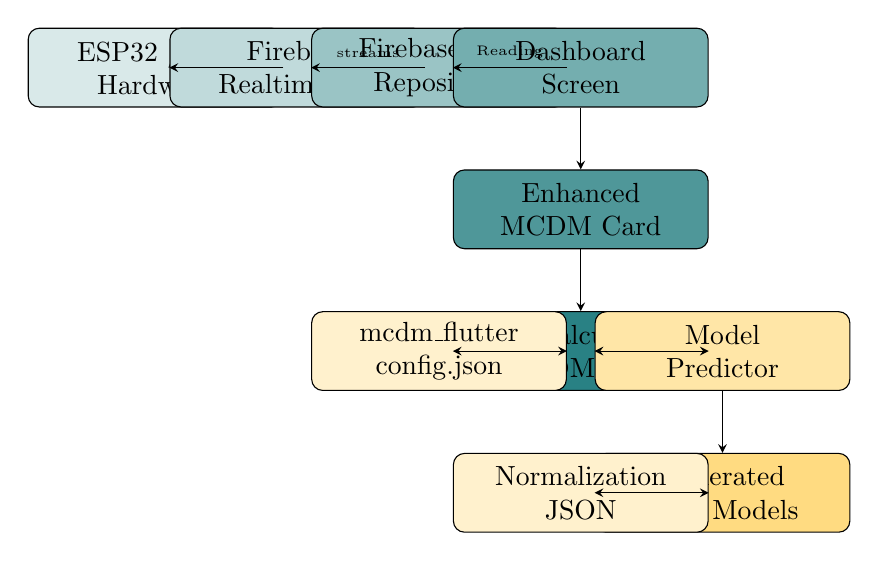
\begin{tikzpicture}[>=stealth, node distance=1.8cm,
    box/.style={draw,rounded corners,fill=teal!20,text width=3cm,align=center,minimum height=1cm}]

    \node[box,fill=teal!15] (esp) {ESP32 / IoT\\Hardware};
    \node[box,fill=teal!25,right of=esp] (fb) {Firebase\\Realtime DB};
    \node[box,fill=teal!40,right of=fb] (repo) {FirebaseData\\Repository};
    \node[box,fill=teal!55,right of=repo] (dash) {Dashboard\\Screen};
    \node[box,fill=teal!70,below of=dash] (widget) {Enhanced\\MCDM Card};
    \node[box,fill=teal!85,below of=widget] (precalc) {PreCalculated\\MCDM Calc};
    \node[box,fill=amber!20,left of=precalc] (config) {mcdm\_flutter\\config.json};
    \node[box,fill=amber!35,right of=precalc] (model) {Model\\Predictor};
    \node[box,fill=amber!50,below of=model] (gen) {Generated\\Dart Models};
    \node[box,fill=amber!20,left of=gen] (norm) {Normalization\\JSON};

    \draw[->] (esp) -- (fb);
    \draw[->] (fb) -- node[above]{\tiny streams} (repo);
    \draw[->] (repo) -- node[above]{\tiny Reading} (dash);
    \draw[->] (dash) -- (widget);
    \draw[->] (widget) -- (precalc);
    \draw[<->] (precalc) -- (config);
    \draw[<->] (precalc) -- (model);
    \draw[->] (model) -- (gen);
    \draw[<->] (gen) -- (norm);
  \end{tikzpicture}
\end{frame}

\begin{frame}[allowframebreaks]{4.10 Key Design Decisions}
  \begin{columns}
    \column{0.5\textwidth}
    \begin{block}{Architecture}
      \textbf{Offline-first:} All MCDM and ML runs locally.
      Firebase is optional (falls back gracefully).

      \vspace{0.2cm}
      \textbf{No server:} ML inference in milliseconds,
      no network latency, works offline.

      \vspace{0.2cm}
      \textbf{Config-driven:} Adding a new dataset = edit JSON,
      add generated model. No code changes to UI.
    \end{block}

    \column{0.5\textwidth}
    \begin{block}{Models \& Math}
      \textbf{Independent MCDM/ML:} Changing weight/scoring
      method does NOT change ML predictions.

      \vspace{0.2cm}
      \textbf{Weight fix:} Models always use
      Compromise+MARCOS internally (best notebook accuracy).

      \vspace{0.2cm}
      \textbf{Pre-calculated weights:} Dynamic weights from
      a single reading are meaningless; notebook-verified
      weights are used instead.
    \end{block}
  \end{columns}
\end{frame}

\begin{frame}[allowframebreaks]{4.11 Project Statistics}
  \centering
  \large \textbf{By the Numbers}

  \vspace{0.5cm}
  \begin{columns}
    \column{0.25\textwidth}
    \begin{block}{\centering Datasets}
      \centering \huge 8
    \end{block}

    \column{0.25\textwidth}
    \begin{block}{\centering Sensors}
      \centering \huge 35+
    \end{block}

    \column{0.25\textwidth}
    \begin{block}{\centering Data Points}
      \centering \huge 154k
    \end{block}

    \column{0.25\textwidth}
    \begin{block}{\centering Dart Files}
      \centering \huge 35+
    \end{block}
  \end{columns}

  \vspace{0.3cm}
  \begin{columns}
    \column{0.25\textwidth}
    \begin{block}{\centering Weight Methods}
      \centering \huge 5
    \end{block}

    \column{0.25\textwidth}
    \begin{block}{\centering Scoring Formulas}
      \centering \huge 4
    \end{block}

    \column{0.25\textwidth}
    \begin{block}{\centering ML Models}
      \centering \huge 8
    \end{block}

    \column{0.25\textwidth}
    \begin{block}{\centering Python Scripts}
      \centering \huge 9
    \end{block}
  \end{columns}

  \vspace{0.3cm}
  \begin{columns}
    \column{0.25\textwidth}
    \begin{block}{\centering Platforms}
      \centering \huge 6
    \end{block}

    \column{0.5\textwidth}
    \begin{block}{\centering Widgets}
      \centering \huge 15
    \end{block}

    \column{0.25\textwidth}
    \begin{block}{\centering Config Lines}
      \centering \huge 1102
    \end{block}
  \end{columns}
\end{frame}

\begin{frame}[allowframebreaks,fragile]{4.12 How to Add a New Dataset}
  \textbf{Step-by-step:} The app is designed for extensibility.

  \vspace{0.3cm}
  \begin{enumerate}
    \item \alert{Creation:} Create your Jupyter notebook with MCDM analysis + ML training
    \item \alert{Train:} Add to \texttt{train\_all\_models.py} --- train and save \texttt{.pkl}
    \item \alert{Export:} Convert to Dart via \texttt{convert\_to\_dart.py} or \texttt{export\_mlp\_to\_dart.py}
    \item \alert{Norm:} Run \texttt{export\_norm\_params.py} to update \texttt{model\_normalization.json}
    \item \alert{Config:} Add dataset entry in \texttt{mcdm\_flutter\_config.json} with sensors, weights, \texttt{modelConfig}
    \item \alert{Dispatch:} Add \texttt{case} in \texttt{ModelPredictor.predict()} for the new dataset ID
    \item \alert{Done:} No UI changes needed! The app reads the config JSON dynamically.
  \end{enumerate}

  \vspace{0.3cm}
  \begin{block}{Example: Adding ``Smart Agriculture'' dataset}
    \begin{itemize}
      \item Add sensors (soil\_moisture, ph, npk) with ranges and modelFeature mappings
      \item Add weights from notebook (5 methods)
      \item Add \texttt{modelConfig} with type ``model'' and class labels
      \item Import generated Dart model, add \texttt{case} in switch
    \end{itemize}
  \end{block}
\end{frame}

\begin{frame}{Summary}
  \centering
  \large \textbf{Your Python foundation + Flutter engineering = Complete IoT monitoring}

  \vspace{0.2cm}
  \begin{columns}[t]
    \column{0.48\textwidth}
    \textbf{You Provided}
    \begin{itemize}
      \item 8 Jupyter notebooks with full MCDM analysis
      \item 40 weight entries (5 methods x 8 datasets)
      \item 8 trained ML models as \texttt{.pkl} files
      \item Domain expertise and dataset curation
    \end{itemize}

    \column{0.48\textwidth}
    \textbf{The App Adds}
    \begin{itemize}
      \item On-device execution (no server needed)
      \item Interactive, real-time visualization
      \item 6-platform deployment target
      \item Config-driven extensibility
      \item 35+ Dart/Service/Widget files, $>$10K lines
    \end{itemize}
  \end{columns}

  \vspace{0.3cm}
  \centering
  \alert{All MCDM math is identical. All ML predictions come from your trained models.\\
  No proxies. No shortcuts. Pure translation.}
\end{frame}

\begin{frame}{Thank You}
  \centering
  \vspace{1cm}
  \Huge \textbf{Questions?}

  \vspace{0.5cm}
  \large \url{https://github.com/anomalyco/opencode}

  \vspace{1cm}
  \small \texttt{env\_reading} --- Environmental IoT Monitoring System
\end{frame}

\end{document}

